\Chapter{Téma elméleti kifejtése}
\label{Chap:tema}

\section {A mesterséges intelligencia}
A mesterséges intelligencia egy viszonylag új, ám hatalmas lehetőségeket rejtő tudományág. A "Mesterséges Intelligencia - Modern megközelítésben" (\cite{bibref:mi_modern}) könyv négy kategóriába sorolja a mesterséges intelligencia mibenlétét, ezen belül is kettő csoportba, amely teljesen más szemszögből vizsgálja a problémát.\ujsor

A megközelítések egyik csoportja az emberközpontú viselkedés, ahol az mesterséges intelligenciától azt várjuk, hogy a lehető legjobban hasonlítson az emberre. Utánozza az emberi gondolkodást az elképzelhető legjobb módon, és cselekvése - amennyire lehet - emberi viselkedésre hasonlítson. A másik megközelítés a racionalitást helyezi középpontba, azaz a mesterséges intelligenciának a rendelkezésre álló információk alapján a lehető legjobb (helyes) döntéseket kell hoznia, és a lehetőségeihez képest a legjobb módon is kell azt végrehajtania. \ujsor

Látszik, hogy ez a két nézőpont teljesen másképpen írja körül a mesterséges intelligencia mibenlétét, ennek megfelelően más módszereket is használ a vizsgálatukra. Matematikai és mérnöki megközelítésben a racionális irányzatok azok ami megfelelően jól vizsgálható ezen tudományok eszköztárával.\ujsor

\subsection{Emberi módon gondolkodni}
Ez az irányzat azt kutatja, hogy hogyan működik az emberi elme, hogy gondolkodik az ember. Ennek kutatására leginkább két módszert használnak: az önelemzést, és a pszichológiai kísérleteket.\ujsor

A mesterséges intelligencia modellezését, és a pszichológiai kísérleteket a kognitív tudomány (más nevén megismeréstudomány) kapcsolja össze. Mivel a kognitív tudomány rendkívül sok, egymástól távol eső tudományterületet foglal magába, ezért célszerűbb kognitív szemléletként hivatkozni rá, nem önálló tudományterület. Foglalkozik - többek között - biológiával, nyelvészettel, számítástechnikával, pszichológiával, és minden olyan tudományággal ami valamilyen módon a megismerési folyamatokat kutatja.\ujsor

Az utóbbi időkben az orvostudomány fejlődésével jobban megismerhettük az agy, illetve a benne található idegsejtek működését, ez inspirálta a mesterséges intelligencia kutatóit a neurális hálók létrehozására és használatára, ami nagyot lendített a természetes nyelv, feldolgozásában, és a gépi látás fejlődésében.

\subsection{Emberi módon cselekedni}
A mesterséges intelligencia - mint tudományág - kialakulásának kezdetén 1950-ben Alan Turing brit matematikus tett egy javaslatot, amivel igazolni lehet egy gépről, hogy intelligensen gondolkodik oly módon, hogy egy szintén intelligens lényhez (ember) mérik összehasonlíthatatlanságukat. Ez afféle munkadefiníció volt, nem kísérelte meg pontosan leírni, hogy egy intelligensen gondolkodó gépnek miféle képességekkel kelljen rendelkezni.\ujsor

A Turing teszt három résztvevőből áll. Egy emberből, egy mesterséges intelligenciából, és egy bírálóból, amelyik szintén ember. A résztvevők egymással írásban kommunikálnak, azonban ezen kívül semmilyen más információt nem ismerhetnek a többiekről. Nem láthatják és nem is hallhatják egymást. A megfigyelő kérdéseket tesz fel felváltva minkét résztvevőnek. Amennyiben a bíráló a feltett kérdéseire kapott válaszból nem tudja egyértelműen megállapítani, hogy melyik résztvevő ember, és melyik a gép, akkor a mesterséges intelligencia teljesítette a Turing-tesztet.\ujsor

Jelenleg nagyon bonyolult lenne egy olyan gépet készíteni amelyik átmenne a \\Turing-teszten, ugyanis képes kell, hogy legyen
\begin{itemize}
	\item Természetes nyelv feldolgozása: A bíráló a kérdéseit valamilyen ember által is beszélt természetes nyelven teszi fel. A kérdést a gépnek meg kell érteni, és ugyanezen a nyelven válaszolnia, ellenkező esetben azonnal lebuktatná magát.
	\item Tanulás: A gép képes kell, hogy legyen új információk elsajátítására, például a bíráló is adhat a gép számára új információt, mely valamely módon visszakérdezhet.
	\item Tudás tárolása: A megszerzett tudást tárolnia kell oly módon, hogy ahhoz\\ könnyen, és gyorsan hozzá tudjon férni szükség esetnén.
	\item Automatizált következtetés: Kérdések megválaszolásához használja fel a megszerzett tudást, illetve vonjon le következtetéseket.
\end{itemize}

Látható, hogy a Turing-teszt kerülte a fizikai kontaktust a résztvevők között, hogy az a bíráló döntését ne befolyásolja, az intelligencia méréshez pedig nincs szükség fizikai kontaktusra. Létezik azonban a kiterjesztett Turing-teszt, amely két további elemmel bővíti a tesztet. Ebben a gépnek videó jelet is fel kell dolgoznia, a látottakra reagálnia kell, továbbá egy nyíláson keresztül tárgyakat átadhat át a bíráló, melyet a gépnek át kell tudnia vennie. (robotika)\ujsor

A teljes Turing-teszt lefedi a mesterséges intelligencia mind a hat ágát, ugyanakkor érte néhány megfontolandó kritika: \cite{bibref:turing}
\begin{itemize}
	\item Nem mindegyik ember képes teljesíteni a tesztet. Gondoljunk itt a valamilyen fogyatékossággal élő emberekre, vagy kisgyerekekre, holott más szempontok alapján ezek az emberek ugyanúgy intelligensnek tekinthetőek.
	\item Elképzelhető, hogy a teszten résztvevő ember megtagadja az együttműködést. Egy valóban emberként viselkedő gép szintén dönthet így, ezáltal megbukik a teszten, holott az együttműködés hiánya nem tekinthető az értelem hiányának
	\item A beszélgetésfolyamat - jellegénél fogva - számos korláttal rendelkezik, ezáltal egy gép megfelelő nagyságú adatbázissal egyszerű mintaillesztéssel képes válaszolni a kérdésekre anélkül, hogy tényleges intelligenciával rendelkezne. 
\end{itemize}

\subsection{Racionálisan gondolkodni} \label{subsection:racional_thinking}
A helyes gondolkodás tudományával már az ókorban is foglalkoztak, Arisztotelész görög filozófus elsőként kísérelt meg általános következtetési folyamatokat törvényekbe foglalni. Később ebből alakult ki a logika tudománya. Ezen ág követői azt remélik, hogy egy logikusan gondolkodó gép minden esetben logikus - azaz - helyes következtetésre jut, ezáltal cselekvése szintén logikus.\ujsor

Az egyik legnagyobb probléma ezzel a megközelítéssel az, hogy az informális tudást a logika formális elemeket használó jelölésrendszerével nehezen kifejezhető, ráadásul sok esetben a tudás helyessége sem garantálható. A másik gond az, hogy egy probléma általában nagyon sok részből, ismeretlenből tevődik össze, amik túl nagy számítási igényt jelentenek.

\subsection{Racionálisan cselekedni}
Az intelligens ágens egyik legfontosabb tulajdonsága, hogy cselekszik, mégpedig olyan módon, hogy a rendelkezésére álló információkból a legjobb döntést hozza meg. A \ref*{subsection:racional_thinking} részben tárgyalt helyes következtetés meghozása csupán az érem egyik oldala. Sokszor kell azonban cselekedni akkor is, ha nem lehetséges helyes következtetést hozni. Vagy azért mert nincsen, vagy pedig azért, mert egyszerűen túl sokáig tartana meghozni a helyes következtetést.

\section{Kétszemélyes teljes információjú játékok}
A kétszemélyes teljes információjú játékok a játékelmélet egy speciális ága. Egy olyan többágenses - egészen pontosan kettő - környezetben játszódik, ahol az ágensek egymás ellenségei, azaz versenyhelyzetben vannak, továbbá cselekvéseiket felváltva hajtják végre.\ujsor

Általában zérus összegű játékokkal foglalkozunk, ami azt jelenti, hogy minden ágens minden cselekedetének hasznossága megegyezik az ellenfélével, csak ellenkező előjellel, tehát arra az előnyre, amit az egyik ágens egy lépésével megtesz, az a másik ágensnek ugyanannyira a hátrányára válik. Fontos megjegyezni, hogy minden kétszemélyes zérus összegű játékban létezik mindkét fél számára optimális stratégia.\ujsor

Teljes információjúnak akkor hívunk egy játékot, ha a játék folyamán - kivéve esetleg az előkészületet - a játéktér minden tekintetben megismerhető az összes ágens számára. Ismerik a játékszabályokat, és az eddig megtett összes lépést.\ujsor

Fontos még megemlíteni, hogy a játszma minden állásában véges - és előre ismert - lépés létezik, továbbá a játszma nem lehet végtelen, azaz véges számú lépés megtétele után az egyik játékos nyer, a másik pedig veszít. (Egyes esetekben a döntetlen végeredmény is elfogadott)

\section{A játékfa}
A kétszemélyes teljes információjú játékok esetében a következő lépés eldöntésének problémájához gyakran alkalmaznak játékfát. A játékfa - mint a neve is mutatja - egy fa adatszerkezet, ami leírja a játék lehetséges állapotait, illetve ezeknek az állapotokban megléphető érvényes lépéseket.\ujsor

A fa csomópontjai a lehetséges állapotok, míg az élek az átmenetet szimbolizálják. A fa szintjei gyakorlatilag egy-egy lépésének felelnek meg, így a vizsgálatot is ennek megfelelően célszerű végezni.\ujsor

Legtöbbször egy már megtalált állapotból nem lehet visszajutni ugyanabba az állapotba - pont ez adja a fa jellegét - ellenkező esetben a fa végtelen nagyságú - ebből következően megoldhatatlan - volna, továbbá sérülne a játék végességére vonatkozó kritérium. Ez probléma főleg az olyan játékokat érinti, ahol a lépések visszavonhatóak, azaz az előzőleg megtett lépés ellentettje a rákövetkező lépésben érvényes lépésnek számít. Amennyiben ilyen előfordul azt többnyire detektálni lehet, és az ilyen ágakat levágják a fát ismét véges nagyságúra - ezáltal a problémát megoldhatóra - redukálva.\ujsor

A megoldás keresése gyakorlatilag a játékfa felépítése, és bejárása. Kezdésként tekintsük a kiinduló állapotot gyökérelemének. Ezután  megvizsgáljuk, hogy végállapotban van-e a játék, majd az összes lehetséges lépést véve egy új ágat hozunk létre, melynek a végére a lépés megtétele utáni állapotteret helyezzük. Egy csomópont további ágainak létrehozását kiterjesztésnek nevezzük. Hogy melyik ággal kezdjük a kiterjesztést azt a keresési stratégia határozza meg. Szükségszerűen a játék végállapotai nem kifejtett csomópontok (levélobjektumok) lesznek.\ujsor

\subsection{Minimax}
Szó esett már arról, hogy miként lehetséges a játékfa felépítése, ám azt még nem részleteztem, hogy miként lehet kiválasztani a soron következő helyes lépést. Ideális esetben egy játékosnak a győzelemhez vezető út a lépések egy sorozata, ám ebbe az ellenfélnek is van beleszólása. Az optimális lépéssorozat kiválasztásában a Minimax (\myref{alg:minimax}) algoritmust tudjuk segítségül hívni.\ujsor

A minimax elv egy kevert stratégia, egy olyan döntési szabály, amely azt célozza meg, hogy minimalizálja a maximális veszteséget, illetve ez meg is fordítható, maximalizálja a minimális nyereséget. \ujsor

\begin{algorithm}
	\caption{Minimax algoritmus pszeudo kódja}
	\label{alg:minimax}
\begin{algorithmic}[1]
	\Function{minimax}{csomopont, melyseg}
	\If {a $csomopont$ levél, vagy $melyseg = 0$}
		\State \Return csomópont heurisztikus értéke
	\Else
		\State $\alpha \gets -\infty$
		\ForAll {gyerekére a csomopontnak}
			\State $\alpha \gets max(\alpha, -\Call{minimax}{gyerek, melyseg - 1})$
			\State \Return $\alpha$
		\EndFor
	\EndIf
	\EndFunction
\end{algorithmic}
\end{algorithm}

Célszerűségből nevezzük el a kezdőjátékost MAX-nak, a második játékost MIN-nek. A minimax elvet a játékfa felépítése során alkalmazzuk. Építsük tehát fel a játékfát az előbb tárgyaltaknak megfelelően, és a végállapotokhoz rendeljünk hozzá egy számértéket. Az olyan játékoknál, ahol csupán azt számít, hogy egy játékos nyert-e elegendő a 1 (MAX nyert), 0 (döntetlen), -1 (MIN nyert) számokkal operálni. Amennyiben a vizsgált játék kifinomultabb pontrendszer rendelkezik, akkor azt az értéket rendeljük hozzá, amennyit az adott játék végállása ér.\ujsor

A megértést segítendő tekintsük a \myref{fig:minimax} játékfát. A MAX játékos lehetséges lépéseit a négyzetek, míg MIN játékosét a rombuszok jelölik. Hogy szemléletesebb legyen a minimax bemutatása jelen játéknál nem csupán az számít, hogy a játékos nyer-e, hanem az is, hogy mennyivel, azaz a MAX a legnagyobb értékre törekszik, míg MIN arra, hogy a MAX-nak legyen a legkevesebb pontja. Az ezt reprezentáló számérték a négyszögek alatt találhatóak, melyek minden lehetséges lépéshez megmutatják a minimax értéket. A szaggatott nyilak a mellettük található számmal minimax lépéseinek a sorrendjét jelölik. A kék a rekurzióba való belépést, míg a pirosak az abból való visszatérést szimbolizálják. Az átláthatóság érdekében a nyilakat csupán az első baloldali részfára helyeztem el, de a számértékeket kiszámítottam minden lépéshez. \ujsor

\begin{figure}[ht]
	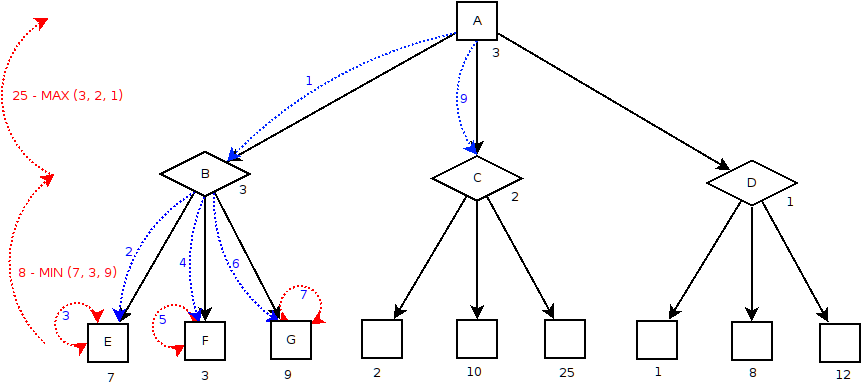
\includegraphics[width=15cm, height=7cm]{minimax}
	\centering
	\caption{Példa a minimax működésére}
	\label{fig:minimax}
\end{figure}

A minimaxot általában rekurzív algoritmussal szokták implementálni, ami ugyan a gyökérelemtől indul ki, de - a rekurziónak köszönhetően - egyből az első levélobjektumot veszi célba. Mivel mindegyik lépés minimax értékét a rákövetkező lépések minimax értékeiből számoljuk ki, ezért a fa legmélyebb pontján kell kezdenünk. A levélobjektum minimax értékének a kiszámítása triviális, ugyanis megegyezik azzal a számértékkel amit a játék végállapotához rendeltünk hozzá. Ezt az ábrán az önmagába visszaforduló nyíllal jelöltem. Nem levélobjektum minimax érték úgy tudjuk kiszámolni, hogy az összes gyerekobjektum minimax értékének vesszük vagy a minimumát, vagy pedig a maximumát attól függően, hogy az adott lépés a MIN, vagy a MAX játékoshoz tartozik-e. Nem meglepő módon a MAX játékos a legnagyobb minimax értékeket keresi, míg a MIN a lehető legkisebbet. Miután egy adott ág egy szintjén kiszámoltuk az összes minimax értéket feljebb léphetünk egy szinttel, ahol ugyan ezeket a lépéseket kell megtennünk, egészen addig, míg vissza nem jutunk a rekurzió legfelsőbb szintjére, a gyökérelemre.\ujsor

Az így felépített játékfa segítségével pedig egyszerűen leolvashatjuk, hogy a MAX-nak milyen lépést kell megtennie: mivel a legnagyobb érték a 4, így a $B$ irányába kell elindulnia, tehát meglépi a $B$ lépést. Ekkor a MIN - ha optimálisan játszik - a legkisebb (jelen esetben szintén a 4) értékhez tartozó lépést, az $F$ lépi meg.\ujsor

Látszik hogy amennyiben a MIN nem játszik optimálisan még rosszabbul jár, ezáltal a minimax algoritmus mindig optimális megoldást ad. A dolog szépséghibája, hogy még az egyszerűbb játékok esetében sem biztos, hogy a MAX-nak lesz elegendő ideje kiszámolni ezt az optimális stratégiát. Ezen a problémán tudnak segíteni a különböző vágási technikák, melyek közül egyet a következő szekcióban be is mutatok.


\section{A játékfa levágásának módszerei}
Az előző részben tárgyaltakat tekintve az olvasóban - jogosan - felmerülhet, hogy a játékfának a használata - még rendkívül egyszerű játékok esetében - is óriási költségekkel (tárhely, számítási igény) jár. A játékfa felépítése minimax algoritmussal $O(b^b)$ idő, és $O(b*m)$ tárigényű, ahol $b$ a csomópontokban létező érvényes lépések $m$ pedig a fa maximális mélysége. Léteznek azonban módszerek, amelyekkel a fa bizonyos részeit le lehet vágni még az előtt, hogy fel kéne építeni, így akár drasztikusan csökkentve ezen költségeket.

\subsection{Alfa-Béta vágás}
Az Alfa-Béta vágás segítségével a gyakorlatban a minimax algoritmust tudjuk felgyorsítani oly módon, hogy a döntésben részt nem vevő ágakat lenyessük, azaz igazából ki sem értékeljük. Ennek megfelelően az alfa-béta vágást a játékfa építése közben kell alkalmazni. A megértés megkönnyítése céljából ezúttal is tekintsünk a már jól ismert \myref{fig:minimax} ábrára. A \myref{alg:alfabeta} algoritmus bemutatja az alfa-béta vágás pszeudokódját.\ujsor

\begin{algorithm}
	\caption{Alfa-Béta vágás algoritmusának pszeudo kódja}
	\label{alg:alfabeta}
	\begin{algorithmic}[1]
		\Function{kiertekel}{csomopont, alfa, beta}
		\If {a $csomopont$ levél}
		\State \Return csomópont heurisztikus értéke
		\EndIf
		\If {a $csomopont$ maximalizálandó}
		\ForAll {gyerekére a csomopontnak}
		\State $\beta \gets MIN(\beta, \Call{kiertekel}{gyerek, alfa, beta})$
		\If {$\beta <= \alpha$}
		\State \Return $\alpha$
		\EndIf
		\EndFor
		\State \Return $\beta$
		\EndIf		
		\If {a $csomopont$ minimalizálandó}
		\ForAll {gyerekére a csomopontnak}
		\State $\alpha \gets MAX(\alpha, \Call{kiertekel}{gyerek, alfa, beta})$
		\If {$\beta <= \alpha$}
		\State \Return $\beta$
		\EndIf
		\EndFor
		\State \Return $\alpha$
		\EndIf	
		\EndFunction
	\end{algorithmic}
\end{algorithm}


Értékeljük ki a minimax értékeket a baloldali részfán az előbb tárgyalt módon, és kezdjük el kiépíteni a második részfát. Láthatjuk, hogy rögtön az első levélobjektumra kiszámított minimax érték kettő, ami már most kisebb, mint az előző részfa utolsó előtti szintjére számított minimális minimax érték. Ez azt jelenti, hogy teljesen felesleges kiszámolnunk jelen részfa további értékeit, hiszen még ha találnánk is nagyobb értéket az utolsó előtti szinten úgyis a minimumot kell vennünk, ami legrosszabb esetben is maga a kettő, ugyanakkor az eggyel feljebb lévő szinten a maximumot keressük, így - mivel a négy nagyobb a kettőnél - a kettő, s ezáltal a teljes $C$ részfa eldobható. Ugyan ez a helyzet a $D$ részfával is. Az alda-béta vágás használatával jelen esetben csupán az első részfát kellett teljesen kiépíteni, a többi részfa az első levélelem minimax számítása után eldobhatóvá vált, s ezzel jelentősen csökkent mind az időigény, mind pedig a tárigény.\ujsor

Természetesen nem minden esetben vagyunk ilyen szerencsések. Látszik, hogy nagyon nem lényegtelen, hogy az ágakat milyen sorrendben értékeljük ki. Sokszor alkalmaznak kiegészítő heurisztikus függvényeket, amelyek megpróbálják megbecsülni a kiértékelés ideális sorrendjét, sőt egyes esetekben - a játék sajátosságaiból adódóan - ez a sorrend előre ismert, vagy kiszámítható. Ez az algoritmus kifejezetten hatékony olyan esetekben, amikor a csomópontoknak sok gyermeke van, és jól meg tudjuk becsülni, hogy melyik az az elem, amelyik elbuktathatja az adott ágat. Ha ezt megtehetjük, akkor az algoritmus időigénye $O(b^{m/2})$-re redukálódik, ami szignifikánsan jobb a minimax $O(b^m)$ időigényétől, ami nagyjából megduplázza a minimax sebességét.

\section{A Nim játék leírása}
A Nim játék egy kétszemélyes teljes információjú körökre osztott stratégiai játék. Egyszeregyből fakadóan számos változata, illetve továbbgondolása is létezik. Néhányat a későbbiekben röviden ismertetni is fogok. \ujsor

A játék körökre bontott, azaz a játékosok felváltva teszik meg lépéseiket. A játék másik lényeges tulajdonsága, hogy teljes információjú játék, azaz a játék kezdetétől fogva mindkét játékos rendelkezésére áll az összes a játékra vonatkozó ismeret. Beleértve a szabályokat, és a teljes játékteret.\ujsor

Nim játék esetében minden kör egy, és csakis egy lépésből áll, amit az éppen soron következő játékosnak kötelezően meg kell tennie. A játéktér tetszőleges számú halomból állhat, melynek elemeinek darabszáma csakugyan kötetlen (lehet egyforma, és akár mindegyik halom eltérő elemszámú). Hagyományosan ezek az elemek kavicsok, de igazából matematikai szempontból ezen entitások manifesztációja lényegtelen. Mindegyik lépés abból áll, hogy az éppen soron következő játékos az egyik nem üres elemszámú halomból elvesz legalább egy, legfeljebb az adott halom elemszámával megegyező darab (tehát akár az egész halmot) entitást a halomból.\ujsor

A játék célja az, hogy amikor sorra kerülünk, akkor ne legyen már több halom, azaz az ellenfelet olyan helyzetbe hozzuk, hogy az végső lépést õ teszi meg, az utolsó entitás(okat) ő veszi el. Ez egyébként a leggyakrabban játszott Nim változat, Misère néven is ismert. Mint már említettem a Nim játéknak számos változata létezik, így előfordul, hogy fordítva játsszák, azaz nem az a soron következő játékos nyer, aki nem tud lépni, hanem az, aki a végső elem(eket) elveszi az utolsó halomból.\ujsor


\section{A Nim játék története}
A Nim játék különböző variációit nagyon régóta játsszák. Pontos információink nincsenek, de egyes források arra engednek következtetni, hogy már az ókori Kínában is játszották ezt a játékot. Ugyancsak erre enged következtetni a \begin{CJK*}{UTF8}{gbsn}捡石子\end{CJK*}
(jiǎn-shízi) kínai eredetű játék, amely kísértetiesen hasonlít a Nim játékra, azzal a kivétellel, hogy ott egy halommal játsszák, igaz ennek is sok variánsa létezik, és az érvényes lépéseknek a szabályai bonyolultabbak. \ujsor
Európában először a 16. század kezdetén tesznek róla említést, de igazán a figyelem középpontjába csak a 19. század végén került, amikor Charles L. Bouton tanulmányozta, majd 1901-ben a játék teljes elméletét kidolgozta. Úgy tudni a játékot is ő keresztelte el Nimnek, a német "Nimm" (elvenni) szó alapján. Más források arra hívják fel a figyelmet, hogy a "NIM" szót 180 fokkal elfordítva az angol "WIN" (nyerni) szót kaphatjuk meg. \ujsor
A játék további ismertségre tett szert az 1939-es New York-i világkiállításon, ahol az 1886-ban alapított amerikai Westinghouse Electric Corporation cég bemutatta a Nimatront, egy olyan gépet, amely Nim játékot játszott. A dolog külön érdekessége, hogy ez volt világon az első elektronikus számítógépes játék.

\section{Ismertebb Nim variációk}
\subsection{Moore-Nim}
A Moore-Nim játék nevét kitalálójáról Eliakim Hastings Moore amerikai matematikusról kapta. Ez egyfajta általánosítása a több-halmos Nim játékoknak, ahol a játékosok egyszerre nem csak egy, hanem legalább egy, maximum $k$ halomból vehetnek el elemeket. Az elvehető elemek számát lehet korlátozni is.

\subsection{Póker-Nim}
A póker-Nimet egy előre rögzített számú entitással játsszák. Kezdetben az összes elemet felhasználva létrehoznak egy normál Nim játékot, majd a játékosok hagyományos Nim játékot játszanak azzal a különbséggel, hogy sorra kerülésükkor nem csupán elvehetnek a halomból, hanem már az elvett elemeket újra felhasználva azokat a halomhoz hozzáadhatják. \ujsor
Könnyen belátható, hogy új elemek hozzáadása a kupachoz nem befolyásolja lényegesen a játékmenetet, hiszen a következő játékos tetszőleges számú elemet elvehet egy kupacból beleértve az előző személy által hozzáadott extra elemeket is.

\subsection{Lasker-Nim}
Nevét az Német-amerikai sakk és Go mesterről Edward Laskerről kapta. Ő javasolta, hogy a hagyományos Nim játékot egészítsék ki egy új érvényes művelettel, a halmok kettébontásával. Ez a kettébontás nem feltétlenül két egyenlő félre való bontást jelent, a két új halom elemszámainak arányára vonatkozóan nincsen megkötés.

\subsection{End-Nim}
End-Nim esetében a halmok sorba vannak rendezve, és bár a játékosok a hagyományos Nim szabályai szerint játszanak, azonban csupán a sor két végén levő halmokból vehetnek el elemeket.

\subsection{Fibonacci-Nim}
Ezt a Nim variánst egyetlen halommal játsszák, de a benne lévő elemek számára nincsen megkötés. A hagyományos Nim játékhoz képest az a különbség, hogy a játékosok legfeljebb mindig az előző játékos által elvett elemek kétszeresét veheti el. A kezdő lépést megtevő játékos tetszőleges (de nem az összes) elemet elvehet a halomból. A kupacból az utolsó entitást elvevő játékos nyer.

\subsection{Wythoff-Nim}
Willem Abraham Wythoff Holland matematikusról kapta a nevét, aki 1907-ben publikálta a játék matematikai analízisét. A játékot két érmehalommal játsszák, minden körben a soron lévő játékosnak el kell vennie valamennyi érmét az egyik kupacból, vagy mindkét halomból egyenlő számú érmét. Az nyer, aki az utolsó érmét, vagy érméket elveszi. \ujsor

A játék megegyezik a királynőt a sarokba játékkal, ahol egy vezért kell eljuttatni valamelyik (általában bal alsó) sarokba, de egy lépés csak akkor érvényes ha azzal közelebb kerül a célhoz.

\subsection{End-Wythoff}
Az egyik legbonyolultabb Nim játék. Ez ötvözi az End-Nim, és a Wythoff-Nim szabályait. Tetszőleges számú halommal játsszák, de a halmok sorba vannak rendezve, és a soron következő játékos csak a szélén lévő halomból vehet el elemeket, vagy a szélén lévő két kupacból megegyező számú elemet.

\subsection{Az osztó játék}
Egy tetszőleges természetes számról indulva a játékosok minden körben elosztják ezt a számot egy olyan prím szám valamely hatványával, amely osztója az éppen aktuális számnak (kivéve természetesen az 1). Az a játékos, amelyik a végén eljut az 1-re, az nyer, vagy veszít attól függően melyik változatát játsszák.

\subsection{A kivonó játék}
Sokan tévesen ezt a variánst ismerik Nim játékként. Többnyire egy halommal játsszák, azonban az elvehető elemek maximális számára van valamilyen $S(1, 2, ..., k)$ korlát.

\subsection{A 21 játék}
Ezt a játékot Misère játékként játsszák. A kezdő mond egy 20-nál kisebb pozitív egész számot, majd a soron következő játékosok az aktuális számot 1, 2, 3-mal növelhetik, de nem léphetik át a 21-et. Az a játékos, amelyik a 21 kimondására kényszerül elveszíti a játszmát.

\subsection{A 100 játék}
A 21 játékhoz nagyon hasonló. Itt a célszám 100, és az azt elérő játékos nyer. A kezdőszám a 0, és a játékosok körönként 1 és 10 közötti egész számot adhatnak hozzá az aktuális értékhez.

\subsection{Körkörös Nim (Kayles)}
Az elemek ebben a variánsban körben helyezkednek el, és a soron következő játékos legfeljebb $k$ egymást követő elemet vehet el a körből. Játszható normál és Misère változatban is.

\subsection{Grundy játéka}
A Grundy játéka egy halommal indul benne tetszőleges számú elemmel. A hagyományos Nim játéktól eltérően itt nem elemeket vesznek el a halomból, hanem a halmokat bontják két nem egyforma méretű halomra. A játéknak akkor van vége, amikor már nincs olyan halom, amit ketté lehetne bontani két nem egyforma méretű halommá. Ezt a variánst is lehet normál, illetve Misère módon játszani.

\subsection{Mohó Nim}
Normális, és Misère módon is játszható a Mohó-Nim, ami csupán annyiban különbözik a hagyományos Nim játéktól, hogy a játékosok csak a legnagyobb elemszámú halomból vehetnek el elemeket.

\subsection{Építő Nim}
Az építő-Nim két részből tevődik össze. Először felépítik Nim játékot az előre megadott számú elemet felhasználva, majd azt lejátsszák. Felépítéskor a játékosok körönként 1-1 elemet raknak (a kezdetben üres) előre meghatározott számú halomba.

\subsection{Northcott-sakk}
A Northcott-sakk egy 8x8-as sakktáblából áll. Kezdetben a játékosok (egymás elől elrejtve) elhelyezik a bábuikat (mindegyik oszlopba csak egyet téve) a saját térfelükön. Miután ezzel végeztek elkezdődik a játék. A játékosok felváltva lépnek, minden körben csak az egyik saját bábujukkal, csak előre, és legfeljebb annyi mezőt, amennyi üres hely van az ő bábuja, és az ellenfél bábuja között, azaz az ellenfél bábuját nem ütheti le, és nem ugorhatja át.\ujsor

\begin{figure}[h]
	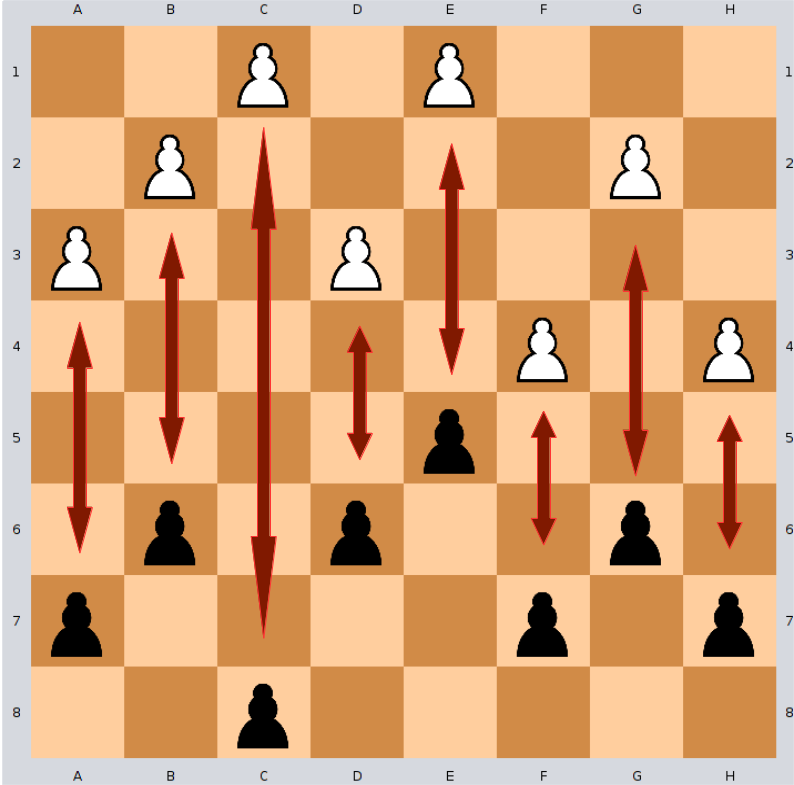
\includegraphics[width=8cm, height=8cm]{northcott-chess}
	\centering
	\caption{Nortcott-sakk táblája. A nyilak a bábuk közti távolságot jelöli, ami a halom méretének feleltethető meg.}
\end{figure}

Ha jobban belegondolunk ez a játék egy az egyben megfeleltethető a hagyományos Nim játéknak, ebből következően játszható sima, és Misère módon is.\ujsor 
Szempontunkból ez a variáns azért is különösen érdekes, mert a szakdolgozatom tartalmazza ennek a játéknak a példaimplementációját, ami ráadásul ténylegesen Nim játékot játszik a háttérben ugyan azt a játékosztályt használva ezzel szemléltetve, hogy mennyire is visszavezethető a Northcott-sakk a standard Nim játékra.

\section{A Nim játék matematikai háttere}
A matematikai háttér elemzését kezdjük néhány definícióval:

\begin{definition}
	Egy nem negatív elemekből álló halmaz legkisebb kizártjának (lkkz) a legkisebb olyan egész számot nevezzük, ami nem szerepel a halmazban.
\end{definition}

\begin{example}
	Például az $A:=\{0, 1, 2, 4, 5, 7, 9\}$ halmaz legkisebb kizártja a 3, mert ez az első olyan nem negatív egész szám, ami nem szerepel az $A$ halmazban.
\end{example}

\begin{definition}
	"Egymással izomorf jólrendezett halmazok közös tulajdonságát nevezzük rendszámnak. Azaz, minden jólrendezett halmaznak van rendszáma és két jólrendezett halmaz rendszáma pontosan akkor azonos, ha izomorfak."
\end{definition}

\begin{remark}
	A fenti definíció a magyar nyelvű Wikipédiáról származik, ez egészen pontosan definiálja a rendszám fogalmát, azonban bevezet sok más fogalmat, melynek a kifejtése meghaladja jelen szakdolgozat témakörét, azonban az angol nyelvű Wikipédia kissé közérthetőbben fogalmaz:
	Halmazelméletben rendszámnak nevezzük a természetes számok koncepciójának egy olyan általánosítását, ami leírja, hogy objektumok egy gyűjteményét hogyan lehet sorrendbe helyezni, egyiket a másik után.
\end{remark}

\begin{definition}
	Nimbereknek (vagy más néven Grundy-számoknak) nevezzük azokat a rendszámokat, amelyeket két további művelettel ruházunk fel. A nimber-összeadással, és a nimber-szorzással.\ujsor
	Nimber-összeadás művelete: $\alpha \oplus \beta = lkkz(\{\alpha' \oplus \beta: \alpha' < \alpha\} \cup \{\alpha \oplus \beta': \beta' < \beta \})$\ujsor
	Nimber-szorzás művelete: $\alpha \beta = lkkz(\{\alpha' \beta + \alpha \beta' + \alpha' \beta': \alpha' < \alpha, \beta' <  \beta\})$
\end{definition}

\begin{remark}
	Számunkra lényeges jelentősége a nimber-összeadásnak van, amelyet számítógépen triviálisan egyszerű implementálni, ugyanis véges rendszámok esetében ez nem más, mint a bitenkénti kizáró vagy, azaz a XOR művelet, melyre a legtöbb processzorban létezik utasítás. 
\end{remark}

Egyszerűség kedvéért vegyünk egy egy halomból álló Nim-játékot. A játék minden lépéséhez rendeljünk hozzá egy nimbert. Ez a szám legyen 0, ha vesztő pozícióban vagyunk, azaz a halomban nincsen elem. Az egy elemű halmaz állapotát az előbbihez képest könnyen meg tudjuk határozni, hiszen egyből csak a nulla pozícióba léphetünk. A legkisebb kizártja ennek a halmaznak az 1, ennek megfelelően rendeljük az egyet a halomhoz. Látható, hogy a kupachoz rendelt nimber megegyezik a halom elemszámosságával. \ujsor

Ezt továbbgondolva kijelenthető, hogy a nimber definíciójából adódóan egy Nim játéknak csak akkor van nyerő stratégiája, ha a játék nimbere nem nulla.

\section{Nyerő stratégia}
Jelen dolgozat írásához végzett irodalomkutatás során sok érdekes, és informatív oldallal találkoztam az interneten. A \cite{bibref:brilliant_nim} internetes oldalon találtam a nyerő stratégiához egy remek leírást bizonyítással egybekötve, amihez úgy érzem nem tudnék érdemben hozzá tenni, ugyanakkor ez a dolgozat bizonyítás nélkül nem lehet teljes, így az alábbiakban közlöm ezen oldalon található angol nyelvű nyerő stratégiájának leírását, illetve annak bizonyítását magyar nyelvre fordítva. Az eredeti bizonyítás Charles L. Boutontól származik, aki elsőként dolgozta ki a Nim játék teljes matematikai hátterét. \cite{bibref:bouton_nim} \ujsor

A nyerő stratégia bemutatását kezdjük egy nagyon fontos definícióval:
\begin{definition}
	Az $a$ és $b$ nemnegatív egész számokon elvégzett $a \oplus b$ műveletet nim-összegnek nevezzük, amennyiben a következő módon kerül kiszámításra. Jelentse $a$ és $b$ kettő különálló hatványainak összegét. Vessük el kettő olyan hatványait, amelyek többször is szerepelnek, majd a fennmaradó hatványokat adjuk össze.
\end{definition}

\begin{remark}
	Ez a definíció gyakorlatilag a nimbereken elvégzett nimber-\\összeadás műveletét írja le kicsit másképpen, de a gyakorlatban ugyan arról van szó. Mint már említettem ez a XOR logikai műveletének felel meg, implementálás során én is ezt használtam ki.
\end{remark}

Például $3 \oplus 5$ a következőképpen számítható ki. A $3 = 2^1 + 2^0$, és az $5 = 2^2 + 2^0$. Mivel a $2^0$ kétszer szerepel, ezért eldobjuk, a maradékot pedig  összeadjuk $2^1 + 2^2$ kiadva az $3 \oplus 5 = 6$ eredményt. \ujsor

Bizonyítható, hogy $\oplus$ asszociatív, ezáltal több szám nim-összegét $a_1 \oplus a_2 \oplus ... \oplus a_n$ definiálja. \ujsor

Legyen egy adott normál Nim állás (a halmok méretei) $a_1, a_2, ... a_n$, az éppen lépő játékos akkor nyer, ha $a_1 \oplus a_2 \oplus ... \oplus a_n \neq 0$; és a nyerő lépést a $i \in \{1, 2, .., n\}$ meghatározásával lehet megtalálni, és a $b_i \in \{0, 1, ..., a_i -1\}$ amivel tehát $a_1 \oplus a_2 \oplus ... \oplus a_{i-1} \oplus b_i \oplus a_{i+1} + a_{i+2} \oplus ... \oplus a_n = 0$ elvéve valamennyi elemet az $i$ halmazból $b_i$ elemet hátrahagyva. Ha $a_1 \oplus a_2 \oplus ... \oplus a_n = 0$, akkor az éppen lépő játékos veszít. \ujsor

Misère Nim esetében a stratégia majdnem teljesen azonos. Egészen addig, amíg a javasolt lépés elvégzése után marad legalább egy halom 2, vagy több elemmel használjuk a normál Nim stratégiáját. Amennyiben a javasolt lépés után nem marad legalább egy halom kettő, vagy több elemmel más lépést kell tennünk:
\begin{itemize}
	\item Ha a javasolt lépés után 1 elem maradna hátra, akkor vegyük el az egész halmot, vagy
	\item Ha a javasolt lépés után nem maradna elem a halomban, úgy hagyjunk benne egy elemet.
\end{itemize}
Más szóval a helyes lépés az, hogy páratlan számú halmokat hagyjunk meg 1 elemmérettel. (Normál esetben páros számú 1 méretű halmokra törekszünk, ezzel a nim-összeget zérussá téve) 


\subsection{Nyerő stratégia bizonyítása}
\begin{theorem}
	A soron következő játékos akkor, és csak akkor nyeri meg a normál Nim játékot, ha a halmok nim-összege nem zérus
\end{theorem}

\begin{proof}
Kezdésnek vegyük az egyszerű alapesetet: ha mindegyik halom elemszáma zérus, akkor a soron következő játékos veszít, és a nim-összeg is zérus. Ettől fogva tegyük fel, hogy nem mindegyik halom üres. \ujsor

Először is vegyük észre, hogy a nim-összeg számos fontos tulajdonsággal rendelkezik. Minden nem negatív a, b, c egész számra igaz, hogy:
\begin{itemize}
	\item Asszociatív: $(a \oplus b) \oplus c = a \oplus (b \oplus c)$
	\item Kommutatív: $a \oplus b = b \oplus a$
	\item Létezik semleges eleme: $0 \oplus a = a$
	\item Öninverz: $a \oplus a = 0$
	\item Lehetséges egyszerre több számnak a Nim-összegét meghatározni oly módon, hogy felírjuk az összes számot 2 különálló hatványaira, majd megkeressük 2 összes olyan hatványát, mely páratlanszor szerepel, végül összeadjuk ezeket 2 hatványokat úgy, hogy mindegyiket csak egyszer vesszük. Például: \ujsor
	$1 \oplus 3 \oplus 7 = (2^0) \oplus (2^0 + 2^1) \oplus (2^0 + 2^1 + 2^2) = 2^0 + 2^2 = 5$
\end{itemize}

Tegyük fel, hogy a halmok elemszáma minden lépés előtt $a_1, a_2, ..., a_n$, illetve \\ $b_1, b_2, ..., b_n$ minden lépés végén. Feltételezzük továbbá, hogy amennyiben $k$ halmon végzünk el egy lépést, akkor minden $i \neq k$ -ra $a_i = b_i$. Legyen $s = a_1 \oplus a_2 \oplus ... \oplus a_n$ és $t_n = b_1 \oplus b_2 \oplus ... \oplus b_n$. Ekkor a következőket kapjuk:
\begin{alignat*}{1}
	t &= 0 \oplus t \\
	&= (s \oplus s) \oplus t \\
	&= s \oplus (s \oplus t) \\
	&= s \oplus ((a_1 \oplus a_2 \oplus ... \oplus a_n) \oplus (b_1 \oplus b_2 \oplus ... \oplus b_n)) \\
	&= s \oplus ((a_1 \oplus b_1) \oplus (a2_ \oplus b_2) \oplus ... \oplus (a_n \oplus b_n)) \\
	&= s \oplus (0 \oplus 0 \oplus ... \oplus 0 \oplus (a_k \oplus b_k) \oplus 0 \oplus ... \oplus 0) \\
	&= s \oplus (a_k \oplus b_k).
\end{alignat*}
Most két eset bizonyítása következik. \ujsor

\begin{lemma}
Ha $s = 0$, akkor $t \neq 0$. Amennyiben az eredeti méretek nim-összege zérus, úgy a lépést végző játékos vesztésre áll (ebből kifolyólag a nim-összeget nem-zérussá kell alakítania)\ujsor
Azt állítjuk, hogy $a_k \oplus b_k \neq 0$. Tegyük fel, hogy így is van, ekkor:

\begin{alignat*}{2}
	a_k &= a_k \oplus 0 \\
	&= a_k \oplus (a_k \oplus b_k) \\
	&= (a_k \oplus a_k) \oplus b_k \\
	&= b_k.
\end{alignat*}

Tehát $a_k = b_k$. De ez ellent mond annak a ténynek, hogy a lépést végrehajtó játékos a $b_k$ halmon végezte el a lépést, s így nem is csökkentette a halom méretét. \ujsor
Tehát mivel $a_k \oplus b_k \neq 0$, így:

\begin{alignat*}{3}
	t &= a \oplus (a_k \oplus b_k) \\
	&= 0 \oplus (a_k \oplus b_k) \\
	&= a_k \oplus b_k \\
	&\neq 0.
\end{alignat*}

\end{lemma}

\begin{lemma}
Ha $s \neq 0$, akkor lehetséges, hogy $t = 0$. Amennyiben  az eredeti halmok nim-összege nem zérus, abban az esetben az éppen lépő játékos nyertes helyzetben van. (hiszen a nim-összeget zérussá tudja alakítani) \ujsor

Vegyük számításba, hogy 2 legmagasabb hatványa $2^k$ nem nagyobb, mint s. Léteznie kell legalább egy olyan $a_i$-nak, ami szintén tartalmazza $2^k$-t, különben $2^k$ nem szerepelhetne s-ben. Most vegyük $b_i = s \oplus a_i$-t. A $b_i$ értéke $2^k$-nal csökken, és legfeljebb $2^{k-1} + 2^{k-2} + ... + 2^0 = 2^k -1 $-gyel nő. (2 minden visszamaradt hatványa kiadja s-t, hozzáadódva az értékhez; például $s = s^2 + 2^1 + 2^0$ és $a_i = 2^3 + 2^2$ kiadja $b_i = 2^3 + 2^1 + 2^0$-t), tehát $b_i < a_i$. Továbbá:
\begin{alignat*}{1}
	t &= s \oplus (a_i \oplus b_i) \\
	&= s \oplus (a_i \oplus (s \oplus a_i)) \\
	&= (s \oplus s) \oplus (a_i \oplus a_i) \\
	&= 0.
\end{alignat*}
\end{lemma}

Ezzel a tétel bizonyítva van.
\end{proof}

